%%%%%%%%%%%%%%%%%%%%%%%%%%%%%%%%%%%%%%%%%
% Beamer Presentation
% LaTeX Template
% Version 1.0 (10/11/12)
%
% This template has been downloaded from:
% http://www.LaTeXTemplates.com
%
% License:
% CC BY-NC-SA 3.0 (http://creativecommons.org/licenses/by-nc-sa/3.0/)
%
%%%%%%%%%%%%%%%%%%%%%%%%%%%%%%%%%%%%%%%%%

%----------------------------------------------------------------------------------------
%	PACKAGES AND THEMES
%----------------------------------------------------------------------------------------

\documentclass[aspectratio=169, hyperref={colorlinks=true,pdfpagelabels=false,linkcolor=black}, xcolor=dvipsnames,10pt]{beamer}
\hypersetup{pdftex=true, colorlinks=true, breaklinks=true, linkcolor=black, menucolor=blue, pagecolor=blue, urlcolor=cyan}


\usepackage{graphicx} % Allows including images
\usepackage{booktabs} % Allows the use of \toprule, \midrule and \bottomrule in tables
\usepackage{xcolor, color}% ,colortbl}
\usepackage{tikz} % nalipour
\usetikzlibrary{tikzmark} % nalipour
\usepackage{hyperref}
\usetikzlibrary{shapes,arrows, decorations.pathreplacing} %nilou
\usetikzlibrary{decorations.markings} %nilou
\usetikzlibrary{trees}%nilou
\usetikzlibrary{decorations.pathmorphing}%nilou
\usepackage{siunitx}%nilou
\usepackage{framed}%nilou
\usetikzlibrary{backgrounds} %nilou
\usepackage[framemethod=tikz]{mdframed}%nilou
\usepackage{adjustbox} %nilou for adjusting the table
\usepackage{amssymb} %nalipour for checkmark
\usepackage{libertine} % For the font

%\usepackage{../../../CLICdp_definitions} % nalipour
\usepackage{xspace}
\usepackage{upgreek} % nalipour
\usepackage{amsmath, mathtools} % nalipour
\renewcommand{\thefootnote}{\fnsymbol{footnote}} % nalipour: symbols
                                % for the footnote
\usepackage{verbatim} % nalipour
\usepackage{fixltx2e}
\usepackage{adjustbox}%nalipour
\usepackage{pifont} %nalipour
\usepackage{smartdiagram}
\usesmartdiagramlibrary{additions}
\usepackage{siunitx}

\usetikzlibrary{angles,quotes}
\usetikzlibrary{positioning}

%%%%%%%%%%%%%%%%%%%%%%%%%%%%%

%----------------------------------------------------------------------------------------
%	TITLE PAGE
%----------------------------------------------------------------------------------------
\title[]{MDI and background studies with IDEA tracker}
\author[Niloufar Alipour Tehrani]{Niloufar Alipour Tehrani \\
on behalf of FCCee MDI group}

\institute[CERN]{}
\date[10 April 2018]{Experiments: Simulation and reconstruction \\    \vspace{0.5cm}
  FCCee Workshop 2019 \\ CERN \\ \vspace{0.3cm}
  10 January 2019}


\setbeamertemplate{navigation symbols}{}
\setbeamertemplate{footline}[frame number]

\usetheme{default}%CambridgeUS}%Boadilla}%Pittsburgh}
\usecolortheme{default}

\setlength{\leftmargini}{2pt} % nalipour: left margin indentation
\renewcommand{\inserttotalframenumber}{\ref{lastframe}}
\begin{document}
\renewcommand{\inserttotalframenumber}{\pageref{lastslide}}

\tikzset{cross/.style={cross out, draw=black, minimum
    size=2*(#1-\pgflinewidth), inner sep=0pt, outer sep=0pt}, %default
  radius will be 1pt.  cross/.default={1pt}}


%%%%%%%%%%%%%%%%%%%%%%%%%%%%%
%         SLIDE             %
%%%%%%%%%%%%%%%%%%%%%%%%%%%%%
\begin{frame}[plain]

  \vspace{1cm}
  \titlepage

  \vspace{-1.5cm}
  \begin{columns}
    \column{0.25\textwidth}
    \centering
    \includegraphics[width=\textwidth]{../logos/FCC-logo}
    \column{0.5\textwidth}
    \column{0.25\textwidth}
    \centering
    \includegraphics[width=0.6\textwidth]{../logos/logo_cern.pdf}
  \end{columns}
\end{frame}



%%%%%%%%%%%%%%%%%%%%%%%%%%%%%
%         SLIDE             %
%%%%%%%%%%%%%%%%%%%%%%%%%%%%%
\begin{frame}
	\frametitle{Introduction}


  \begin{itemize}
  \item The current status of the simulation of the IDEA
    detector with FCCSW
  \item Validation of the detector
  \item Study of the impact of beam-background on the IDEA
    drift chamber
  \item Few investigations for the tracking
  \end{itemize}

    \begin{block}{FCCSW: FCC Software}
      \begin{itemize}
      \item Common software for all FCC experiments
        \begin{itemize}
        \item ee, hh \& eh
        \end{itemize}
      \item Detector and physics studies
        \begin{itemize}
        \item Fast \& full simulations
        \item One software stack from event generation to physics analysis
        \end{itemize}
      \item Collaborative approach
      \end{itemize}
    \end{block}

%
% \column{0.3\textwidth}
% \centering
% \includegraphics[width=\textwidth]{../figures/cernFCC}


\end{frame}


%%%%%%%%%%%%%%%%%%%%%%%%%%%%%
%         SLIDE             %
%%%%%%%%%%%%%%%%%%%%%%%%%%%%%
\begin{frame}
  \frametitle{The IDEA detector concept for FCC-ee}

  \begin{itemize}
    \item The IDEA detector is one of the two detector concepts for the FCC-ee
  \end{itemize}

  \begin{columns}
    \column{0.5\textwidth}
      \begin{itemize}
        \item Main features of the IDEA concept
          \begin{itemize}
            \item Vertex detector: MAPS
            \item Ultra-light drift chamber with particle identification
            \item Dual-readout calorimetry
            \item Aditional silicon disk layers placed in the space between the drift chamber and the dual readout calorimeter to serve as a precise tracking layer and a pre showering device
            \item 2~T axial magnetic field
            \item Instrumented return yoke
          \end{itemize}
      \end{itemize}

    \column{0.5\textwidth}
      \centering
      \includegraphics[width=\textwidth]{./figures/FCCeeIDEAConcept}

  \end{columns}

\end{frame}


%%%%%%%%%%%%%%%%%%%%%%%%%%%%%
%         SLIDE             %
%%%%%%%%%%%%%%%%%%%%%%%%%%%%%
\begin{frame}
  \frametitle{Give it a try!}

  \url{https://github.com/HEP-FCC/FCCSW}

  \centering
  \includegraphics[width=\textwidth]{figures/IDEAweb}

\end{frame}

%%%%%%%%%%%%%%%%%%%%%%%%%%%%%
%         SLIDE             %
%%%%%%%%%%%%%%%%%%%%%%%%%%%%%
\begin{frame}
  \frametitle{The IDEA detector as visualized with FCCSW}

  \centering
  \begin{tikzpicture}
    \node[anchor=south west,inner sep=0] (image) at
    (0,0){\includegraphics[width=0.9\textwidth]{figures/FCCeeIDEA_IR}};
    \begin{scope}[x={(image.south east)},y={(image.north west)}]
    \node[left] at (0.6, 0.7) {\textbf{Drift Chamber}};

    \draw[->, thick](0.05, 0.25) -- (0.05, 0.1);
    \node[above] at (0.05, 0.25) {\textbf{Beam Pipe}};

    \draw[->, thick](0.15, 0.45) -- (0.15, 0.22);
    \node[above] at (0.15, 0.45) {\textbf{Solenoid Shielding}};

    \draw[->, thick](0.2, 0.7) -- (0.42, 0.4);
    \node[above] at (0.2, 0.7) {\textbf{Tungsten Shielding}};

    \draw[->, thick](0.55, 0.05) -- (0.48, 0.4);
    \node[below] at (0.55, 0.05) {\textbf{Luminosity Calorimeter}};

    \draw[->, thick](0.75, 0.2) -- (0.58, 0.5);
    \node[below] at (0.75, 0.2) {\textbf{Vertex Detector}};

  \end{scope}
  \end{tikzpicture}

\end{frame}

%%%%%%%%%%%%%%%%%%%%%%%%%%%%%
%         SLIDE             %
%%%%%%%%%%%%%%%%%%%%%%%%%%%%%
\begin{frame}
  \frametitle{The IDEA drift chamber}

  \begin{columns}
  \column{0.6\textwidth}
    \begin{itemize}
      \item The parameters of the drift chamber \vspace{0.5cm}
    \end{itemize}

    \centering
    \begin{adjustbox}{max width=1\textwidth}
      \begin{tabular}{l l}
        \toprule
          Gas & $90~\%$ Helium \&\\
          & $10~\%$ isobutane ($\text{C}_{4}\text{H}_{10}$) \\
          Length & 4~m \\
          Inner radius & 0.345~m \\
          Outer radius & 2~m\\
          Nb. layer & 112 \\
          Cell size & 12~mm - 14.7~mm \\
          Number of sensitive wires & 56'448 \\
          Transverse resolution & 0.1~mm \\
          Longitudinal resolution & 1~mm \\
        \bottomrule
      \end{tabular}
    \end{adjustbox}

  \column{0.4\textwidth}
    \centering
    \includegraphics[width=\textwidth]{Figures/Field_sensWires.png}

  \end{columns}

  \begin{itemize}
    % \item The gas volume is divided into a set of hyperboloid layers.
    % \item Each layer contains single sense wire cells.
    \item Field wires surround the sense wires to provide homogeneous electric field for each cell.
    \item The wires are rotated with an average stereo angle of 0.1~radians to improve the longitudinal resolution along them.
  \end{itemize}


\end{frame}


%%%%%%%%%%%%%%%%%%%%%%%%%%%%%
%         SLIDE             %
%%%%%%%%%%%%%%%%%%%%%%%%%%%%%
\begin{frame}
  \frametitle{The simulation chain in FCCSW}

  \begin{enumerate}
  	\item Detector geometry description with DD4hep
  		\begin{itemize}
  		\item Collaborative effort with CLIC, ILC and LHCb
  		\item The IR region and the VXD from CLD are as well implemented in DD4hep
  		\item Definition of the gas layers in the DCH (with hyperboloid volumes)
  		\end{itemize}
  	\item Segmentation of the sensitive areas
  		\begin{itemize}
  		\item Information on the position of the sense wires instead of placing physical volumes
  		\item Speeds up the simulation
  		\end{itemize}
  	\item Geant4 simulation
  		\begin{itemize}
  		\item Calculate the E\textsubscript{dep} for each ionisation action
  		\item Charge drift to the wires
  		\end{itemize}
  	\item Hit reconstruction
  		\begin{itemize}
  		\item Combination of individual hit calculations from (3)
  		\item Calculation of the signal in the wire
  		\end{itemize}
    \item Track reconstruction with ACTS \textcolor{Green}{$\Rightarrow$ under investigation}
	\end{enumerate}

  \centering
  \smartdiagramset{back arrow disabled=true}
  \usebeamercolor{background canvas}
    \smartdiagram[flow diagram:horizontal]
    {%
      {Geometry\\DDhep}, Segmentation, {Geant4 \\simulation}, Hit Reconstruction, Tracking%
    }

\end{frame}

%%%%%%%%%%%%%%%%%%%%%%%%%%%%%
%         SLIDE             %
%%%%%%%%%%%%%%%%%%%%%%%%%%%%%
\begin{frame}
  \frametitle{The simulation of the drift chamber using FCCSW}


  \begin{columns}
  \column{0.5\textwidth}
    \begin{itemize}
      \item The sensitive wires as simulated in the first layer of the drift chamber with FCCSW.
      \item The DD4hep segmentation (\textsc{DDSegmentation}) is responsible to associate a hit to the wire it drifts to
        \begin{itemize}
          \item Reduces the running time by avoiding to place each wire individually
        \end{itemize}
    \end{itemize}

    \centering
    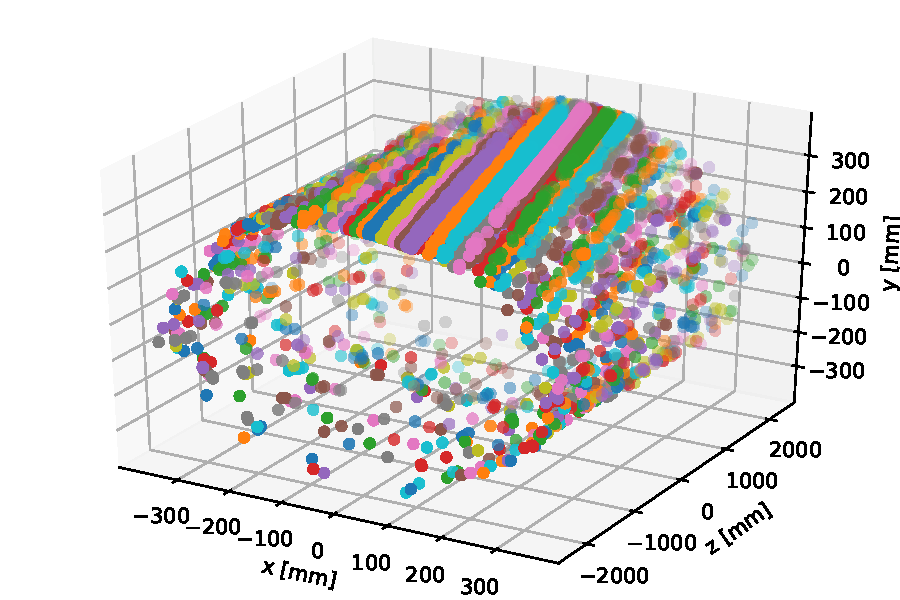
\includegraphics[width=0.9\textwidth]{figures/allHits}

    \column{0.5\textwidth}
    \begin{itemize}
      \item The coverage of the drift chamber as a function of the polar angle $\theta$ is investigated.
      \item High coverage in the barrel region by $\sim 112$ wires in average.
      \item In the forward region, silicon disks are foreseen to improve the track angle coverage.
    \end{itemize}

    \vspace{-0.1cm}
    \centering
    \includegraphics[width=0.9\textwidth]{figures/numWires}

  \end{columns}

  %
  % \begin{columns}
  %   \column{0.5\textwidth}
  %   \begin{itemize}
  %     \item The coverage of the drift chamber as a function of the polar angle $\theta$ is investigated. \vspace{0.5cm}
  %     \item High coverage in the barrel region by $\sim 112$ wires in average. \vspace{0.5cm}
  %     \item In the forward region, silicon disks are foreseen to improve the track angle coverage. \vspace{0.5cm}
  %   \end{itemize}
  %
  %   \column{0.5\textwidth}
  %     \centering
  %     \includegraphics[width=\textwidth]{figures/numWires}
  % \end{columns}

\end{frame}


%%%%%%%%%%%%%%%%%%%%%%%%%%%%%
%         SLIDE             %
%%%%%%%%%%%%%%%%%%%%%%%%%%%%%
\begin{frame}
  \frametitle{Beam-induced backgrounds at FCC-ee}

  \begin{itemize}
    \item Three main sources of beam-induced backgrounds at FCC-ee
    \begin{itemize}
      \item \textbf{Incoherent $e^+e^-$ pairs} due to bremstrahlung photons $\Rightarrow$ highest source of background
      \item \textbf{$\gamma\gamma\rightarrow$ hadrons} $\Rightarrow$ Expected to have a very low impact
      \item \textbf{Synchrotron radiation (SR)} $\Rightarrow$ Dictates the design of the interaction region (IR)
        \begin{itemize}
          \item Defines the beampipe radius, the design of the shielding (in Tungesten)
          \item Mostly stopped by the shielding, few SR photons can hit the detector
        \end{itemize}
    \end{itemize}
  \end{itemize}

  \begin{columns}
    \column{0.5\textwidth}
      \begin{itemize}
        \item The trajectory of the $e^+e^-$ pairs in a 2~T magnetic field (using helix extrapolation).

        \item No direct hits in the drift chamber (with inner radius of 345~mm)
      \end{itemize}

    \column{0.5\textwidth}
      \centering
      \includegraphics[width=\textwidth]{./figures/pairs_R_Z}

    \end{columns}

\end{frame}

%%%%%%%%%%%%%%%%%%%%%%%%%%%%%
%         SLIDE             %
%%%%%%%%%%%%%%%%%%%%%%%%%%%%%
\begin{frame}
  \frametitle{The impact of the incoherent background pairs}

  \begin{columns}

    \column{0.5\textwidth}
    \begin{itemize}
      \item $e^+e^-$ pairs is the background with the highest Impact
      \item The occupancy is defined as the percentage of wires hits per layer
      \item The average bunch spacing
        \begin{itemize}
          \item At the Z stage ($\sqrt{s}=$91.2~GeV): 19.6~ns
          \item At the top stage ($\sqrt{s}=$365~GeV): 3396~ns
        \end{itemize}
      \item At the Z stage, the background is integrated over 4 BX to take into account the readout time for the signal.
    \end{itemize}

    \column{0.5\textwidth}
    \centering
    \includegraphics[width=\textwidth]{Figures/incoherent_top_Z.pdf}

  \end{columns}

\end{frame}

%%%%%%%%%%%%%%%%%%%%%%%%%%%%%
%         SLIDE             %
%%%%%%%%%%%%%%%%%%%%%%%%%%%%%
\begin{frame}
  \frametitle{Conclusions on the beam-induced backgrounds}

  \centering
  \begin{adjustbox}{max width=\textwidth}
    \begin{tabular}{l c c}
      \toprule
       Background & \multicolumn{2}{c}{Average occupancy} \\
        & $\sqrt{s}$ = 91.2~GeV & $\sqrt{s}$ = 365~GeV \\
       \midrule
       $e^+e^-$ pair background & 1.1\% & 2.9\% \\
       $\gamma\gamma\rightarrow$ hadrons & 0.001\% & 0.035\%  \\
       Synchrotron radiation & negl. & 0.2\% \\
       \bottomrule
    \end{tabular}
  \end{adjustbox}

  \vspace{0.8cm}

  \begin{itemize}
    \item Based on experience from the MEG2 drift chamber, this is believed to be a manageable level.
    \item Exploiting the power of the drift chamber timing measurement, the background level can be greatly reduced.
    \item The track reconstruction in the presence of the beam-induced background needs to be investigated with the current simulation tools.
  \end{itemize}

\end{frame}


%%%%%%%%%%%%%%%%%%%%%%%%%%%%%
%         SLIDE             %
%%%%%%%%%%%%%%%%%%%%%%%%%%%%%
\begin{frame}
  \frametitle{Tracking \& FCCSW}

  \begin{columns}
    \column{0.5\textwidth}
    \begin{itemize}
      \item ACTS: A Common Tracking Software
      \item High-level track reconstruction modules to be used for any tracking detector
      \item Ultimate goal for tracking in FCCSW
    \end{itemize}

    \column{0.5\textwidth}
    \centering
    \includegraphics[width=0.5\textwidth]{Figures/ACTSlogo.png}
  \end{columns}

  \begin{itemize}
    \item Implementations needed for the DCH
      \begin{itemize}
        \item The geometry (wires, rotations with the stereo angle)
        \item In the extrapolation step, a new strategy to manage the high number of wires to limit the computation time (ex. navigation, ...)
      \end{itemize}
    \item For FCCSW, the Tricktrack software provides the seeding algorithms (initially implemented for FCC-hh and based on the CMS tracking software)
  \end{itemize}

\end{frame}

%%%%%%%%%%%%%%%%%%%%%%%%%%%%%
%         SLIDE             %
%%%%%%%%%%%%%%%%%%%%%%%%%%%%%
\begin{frame}
  \frametitle{Tracking: Hough transform}

  \begin{itemize}
    \item Before tackling ACTS, a faster solution is to use the Hough transform
    \item Used for feature extraction in image analysis, computer vision, ...
      \begin{itemize}
        \item Identification of lines, ellipses, circles
      \end{itemize}
    \item Initially invented for the analysis of bubble chamber photographs
    \item A possible solution for the drift chamber
    \begin{itemize}
      \item Use Tricktrack for seeding in the VXD and limit the search region in the drift chamber.
      \item Hough Transform for pattern recognition $\Rightarrow$ track reconstruction efficiency
      \item The track parameters are obtained by using the extrapolation algorithms provided by ACTS or Tricktrack
    \end{itemize}
  \end{itemize}

\end{frame}

%%%%%%%%%%%%%%%%%%%%%%%%%%%%%
%         SLIDE             %
%%%%%%%%%%%%%%%%%%%%%%%%%%%%%
\begin{frame}
  \frametitle{Example: detecting a simple line}

  \begin{columns}
    \column{0.7\textwidth}
    \begin{itemize}
      \item Represented as a point (b, m) in the parameter space
    \end{itemize}
    \begin{equation}
      y = m \cdot x + b
    \end{equation}

    \begin{itemize}
      \item Hough space: (r, $\theta$)
    \end{itemize}
    \begin{equation}
      r = x \cdot \cos(\theta) + y \cdot \sin(\theta)
    \end{equation}

    \column{0.3\textwidth}
      \centering
      \includegraphics[width=0.8\textwidth]{figures/linepic}

  \end{columns}

  \begin{itemize}
    \item A line corresponds to local maxima in the Hough space.
  \end{itemize}

  \begin{columns}
    \column{0.5\textwidth}
      \centering
      \includegraphics[width=0.8\textwidth]{figures/line.pdf}

    \column{0.5\textwidth}
      \centering
      \includegraphics[width=0.8\textwidth]{figures/line_hough.pdf}
  \end{columns}

\end{frame}

%%%%%%%%%%%%%%%%%%%%%%%%%%%%%
%         SLIDE             %
%%%%%%%%%%%%%%%%%%%%%%%%%%%%%
\begin{frame}
  \frametitle{A track in a magnetic field}

\begin{columns}
  \column{0.5\textwidth}

  \begin{itemize}
    \item Parametrization by a helix
    \begin{itemize}
      \item $\phi_0$: initial azimuthal angle
      \item $d_0$: distance of closest approach
      \item $r_{T,0}$: the radius of the track
      \item $\theta_0$: the initial polar angle
      \item $z_0$: the initial z-coordinate at the point of closest approach
    \end{itemize}
    \item Algorithm:
    \begin{itemize}
      \item Map a helix trajectory into a straight line (conformal transform)
      \item Find track parameters in the Hough space
      \item Computation of the track parameters
    \end{itemize}
    \item Reference $\rightarrow$ DOI: \url{10.1051/epjconf/201715000014}
  \end{itemize}

  \column{0.5\textwidth}
    \centering
    \includegraphics[width=0.7\textwidth]{Figures/helix_param_1.png} \\
    \hspace{0.8cm}
    \includegraphics[width=0.7\textwidth]{Figures/helix_param_2.png}

  \end{columns}

\end{frame}

%%%%%%%%%%%%%%%%%%%%%%%%%%%%%
%         SLIDE             %
%%%%%%%%%%%%%%%%%%%%%%%%%%%%%
\label{lastslide}
\begin{frame}
  \frametitle{Summary \& Outlook}


  \begin{itemize}
    \item The IDEA detector well integrated within FCCSW
    \item The impact of the beam-induced backgrounds on the drift chamber is studied
      \begin{itemize}
        \item Estimation of the occupancy
        \item Reasonable based on past experience with the drift chamber for MEG2
      \end{itemize}
    \item Investigation on the tracking $\Rightarrow$ methods to be implemented soon.
  \end{itemize}

  \vspace{1cm}
	\centering
	\Large{\textbf{Thank you for your attention!}}
\end{frame}

%%%%%%%%%%%%%%%%%%%%%%%%%%%%%
%         SLIDE             %
%%%%%%%%%%%%%%%%%%%%%%%%%%%%%
\begin{frame}

	\centering
	\Huge{Backup slides}
\end{frame}

%%%%%%%%%%%%%%%%%%%%%%%%%%%%%
%         SLIDE             %
%%%%%%%%%%%%%%%%%%%%%%%%%%%%%
\begin{frame}
	\frametitle{The dimensions of the vertex \& tracking detectors}


  \begin{itemize}
	\item FCCee\_o1\_v02
	\end{itemize}

	\begin{tabular}{l|l|l}
	Parameters & FCCee (Si) & FCCee (IDEA) \\ \hline
	VXD Barrel r\textsubscript{in} & \textcolor{Green}{17 mm} & \textcolor{Green}{17 mm} \\
	VXD Barrel r\textsubscript{out} & 59 mm & 59 mm \\
	VXD Barrel length & 250 mm & 250 mm \\
	VXD Endcap r\textsubscript{in} & 24 - 45 mm & 24 - 45 mm \\
	VXD Endcap r\textsubscript{out} & 102 mm & 102 mm \\
	VXD Endcap z\textsubscript{position} & 159-301 mm & 159-301 mm \\
	Tracker Barrel r\textsubscript{in} & \textcolor{Green}{127 mm} & \textcolor{Green}{345 mm} \\
	Tracker Barrel r\textsubscript{out} & \textcolor{Green}{2100 mm} & \textcolor{Green}{2000 mm} \\
	Tracker Barrel length & 2528 mm & 4500 mm \\
	Tracker Endcap r\textsubscript{in} & 78 mm & N.A. \\
	Tracker Endcap r\textsubscript{Out} & 2080 mm & N.A. \\
	Tracker Endcap z\textsubscript{pos} range & 524:2190 mm & N.A. mm \\
	\end{tabular}


\end{frame}

%----------------------------------------------------------------------------------------
%	End of Document
%----------------------------------------------------------------------------------------
\end{document}
